\begin{figure}[h!]
\begin{center}
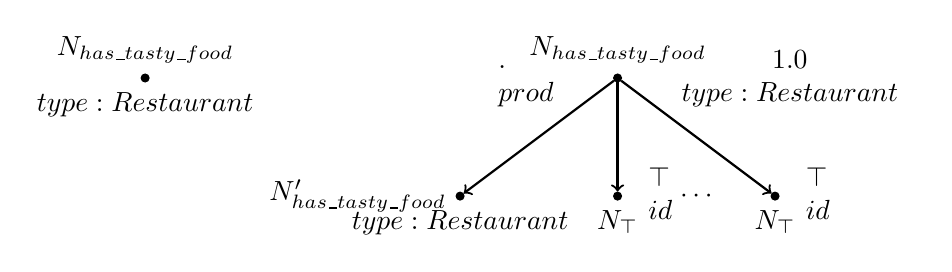
\begin{tikzpicture}[yscale=-1,
place/.style={circle,draw=black, fill=black, inner sep=0pt, 
              minimum size=1mm}]

 \node[place] (1st) at (0, 0) [label=above: $N_{has\_tasty\_food}$,
                               label=below: $type : Restaurant$] {};
	

\begin{scope}[xshift=4cm]
  \node[place] (1st) at (2, 0) [label=above: $N_{has\_tasty\_food}$,
                                label=right: 
       \begin{tabular}{l c}
         & $1.0$\\
         & $type : Restaurant$ \\
       \end{tabular},
       label=left:
       \begin{tabular}{l l}
         $.$ &\\
         $prod$ &\\
       \end{tabular}] {};
  \node[place] (2nd) at (0, 1.5) [label=left: $N'_{has\_tasty\_food}$,
                                  label=below: $type : Restaurant$] {};
  \node[place] (3rd) at (2, 1.5) [label=below: $N_{\top}$,
  						  label=right: 
             \begin{tabular}{l}
            $\top$\\
            $id$\\
             \end{tabular}
	]{}; 

  \node[place] (4th) at (4, 1.5) [label=below: $N_{\top}$,
    						  label=right: 
             \begin{tabular}{l}
            $\top$\\
            $id$\\
             \end{tabular}
  ]{};

  \node (dots) at (3,1.5) {$\cdots$};

  \draw[->, thick] (1st) -- (2nd);
  \draw[->, thick] (1st) -- (3rd);
  \draw[->, thick] (1st) -- (4th);
\end{scope}

\end{tikzpicture}
\end{center}   
\caption{two equivalent predicate trees for has\_tasty\_food}
\label{fig:ex1}
\end{figure}